\chapter{基于深度学习方法的低分辨率环境下微表情识别}\label{chap:owner2}

% 为方便使用及更好地展示\LaTeX{}排版的优秀特性,ucasthesis的框架和文件体系进行了细致地处理,尽可能地对各个功能和板块进行了模块化和封装,对于初学者来说,众多的文件目录也许一开始让人觉得有些无所适从,但阅读完下面的使用说明后,会发现原来使用思路是简单而清晰的,而且,当对\LaTeX{}有一定的认识和了解后,会发现其相对Word类排版系统极具吸引力的优秀特性。所以,如果是初学者,请不要退缩,请稍加尝试和坚持,以领略到\LaTeX{}的非凡魅力,并可以通过阅读相关资料如\LaTeX{} Wikibook\citep{wikibook2014latex}来完善自己的使用知识。

\section{数据增强}

% \begin{enumerate}
%     \item 安装软件:根据所用操作系统和章节~\ref{sec:system}中的信息安装\LaTeX{}编译环境。
%     \item 获取模板:下载 \href{https://github.com/mohuangrui/ucasthesis}{ucasthesis} 模板并解压。ucasthesis模板不仅提供了相应的类文件,同时也提供了包括参考文献等在内的完成学位论文的一切要素,所以,下载时,推荐下载整个ucasthesis文件夹,而不是单独的文档类。
%     \item 编译模板:
%         \begin{enumerate}
%             \item Windows:双击运行artratex.bat脚本。
%             \item Linux或MacOS: {\scriptsize \verb|terminal| -> \verb|chmod +x ./artratex.sh| -> \verb|./artratex.sh xa|}
%             \item 任意系统:都可使用\LaTeX{}编辑器打开Thesis.tex文件并选择xelatex编译引擎进行编译。
%         \end{enumerate}
%     \item 错误处理:若编译中遇到了问题,请先查看“常见问题”(章节~\ref{sec:qa})。
% \end{enumerate}
%
% 编译完成即可获得本PDF说明文档。而这也完成了学习使用ucasthesis撰写论文的一半进程。什么?这就学成一半了,这么简单???,是的,就这么简单!

\subsection{数据集混合}

% Thesis.tex为主文档,其设计和规划了论文的整体框架,通过对其的阅读可以了解整个论文框架的搭建。

\subsection{直方图均衡化}

% \begin{itemize}
%     \item Windows:双击Dos脚本artratex.bat可得全编译后的PDF文档,其存在是为了帮助不了解\LaTeX{}编译过程的初学者跨过编译这第一道坎,请勿通过邮件传播和接收此脚本,以防范Dos脚本的潜在风险。
%     \item Linux或MacOS:在terminal中运行
%         \begin{itemize}
%             \item \verb|./artratex.sh xa|:获得全编译后的PDF文档
%             \item \verb|./artratex.sh x|:快速编译模式
%         \end{itemize}
%     \item 全编译指运行 \verb|xelatex+bibtex+xelatex+xelatex| 以正确生成所有的引用链接,如目录,参考文献及引用等。在写作过程中若无添加新的引用,则可用快速编译,即只运行一遍\LaTeX{}编译引擎以减少编译时间。
% \end{itemize}

\subsection{亮度调整}

% 运行编译脚本后,编译所生成的文档皆存于Tmp文件夹内,包括编译得到的PDF文档,其存在是为了保持工作空间的整洁,因为好的心情是很重要的。
\section{P3D ResNet}

在视频分类或理解领域,容易从图像领域的2D卷积联想到用3D卷积来做,虽然用3D卷积进行特征提取可以同时考虑到spatial和temporal维度的特征,但是计算成本和模型存储都太大,因此这篇文章针对视频领域中采用的3D卷积进行改造,提出Pseudo-3D Residual Net (P3D ResNet),思想有点像当年的Inception v3中用1*3和3*1的卷积叠加代替原来的3*3卷积,这篇文章是用1*3*3卷积和3*1*1卷积代替3*3*3卷积(前者用来获取spatial维度的特征,实际上和2D的卷积没什么差别;后者用来获取temporal维度的特征,因为倒数第三维是帧的数量),毕竟这样做可以大大减少计算量,而如果采用3D卷积来做的话,速度和存储正是瓶颈,这也使得像C3D算法的网络深度只有11层,参看Figure1。该文章的网络结构可以直接在3D的ResNet网络上修改得到。顺便提一下,除了采用3D卷积来提取temporal特征外,还可以采用LSTM来提取,这也是当前视频研究的一个方向。

Figure1是几个模型在层数、模型大小和在Sports-1M数据集上的视频分类效果对比,其中的P3D ResNet是在ResNet 152基础上修改得到的,深度之所以不是152,是因为改造后的每个residual结构不是原来ResNet系列的3个卷积层,而是3或4个卷积层,详细可以看Figure3,所以最后网络深度是199层。官方github代码中的网络就是199层的。ResNet 152是直接在Sports-1M数据集上fine tune得到的。可以看出199层的P3D ResNet虽然在模型大小上比ResNet-152(此处ResNet-152是在sports-1M数据集上fine tune得到的)大一些,但是准确率提升比较明显,与C3D(此处C3D是直接在sports-1M数据集上从头开始训练得到的)的对比在效果和模型大小上都有较大改进,除此之外,速度的提升也是亮点,后面有详细的速度对比。

\begin{figure}[]
\centering
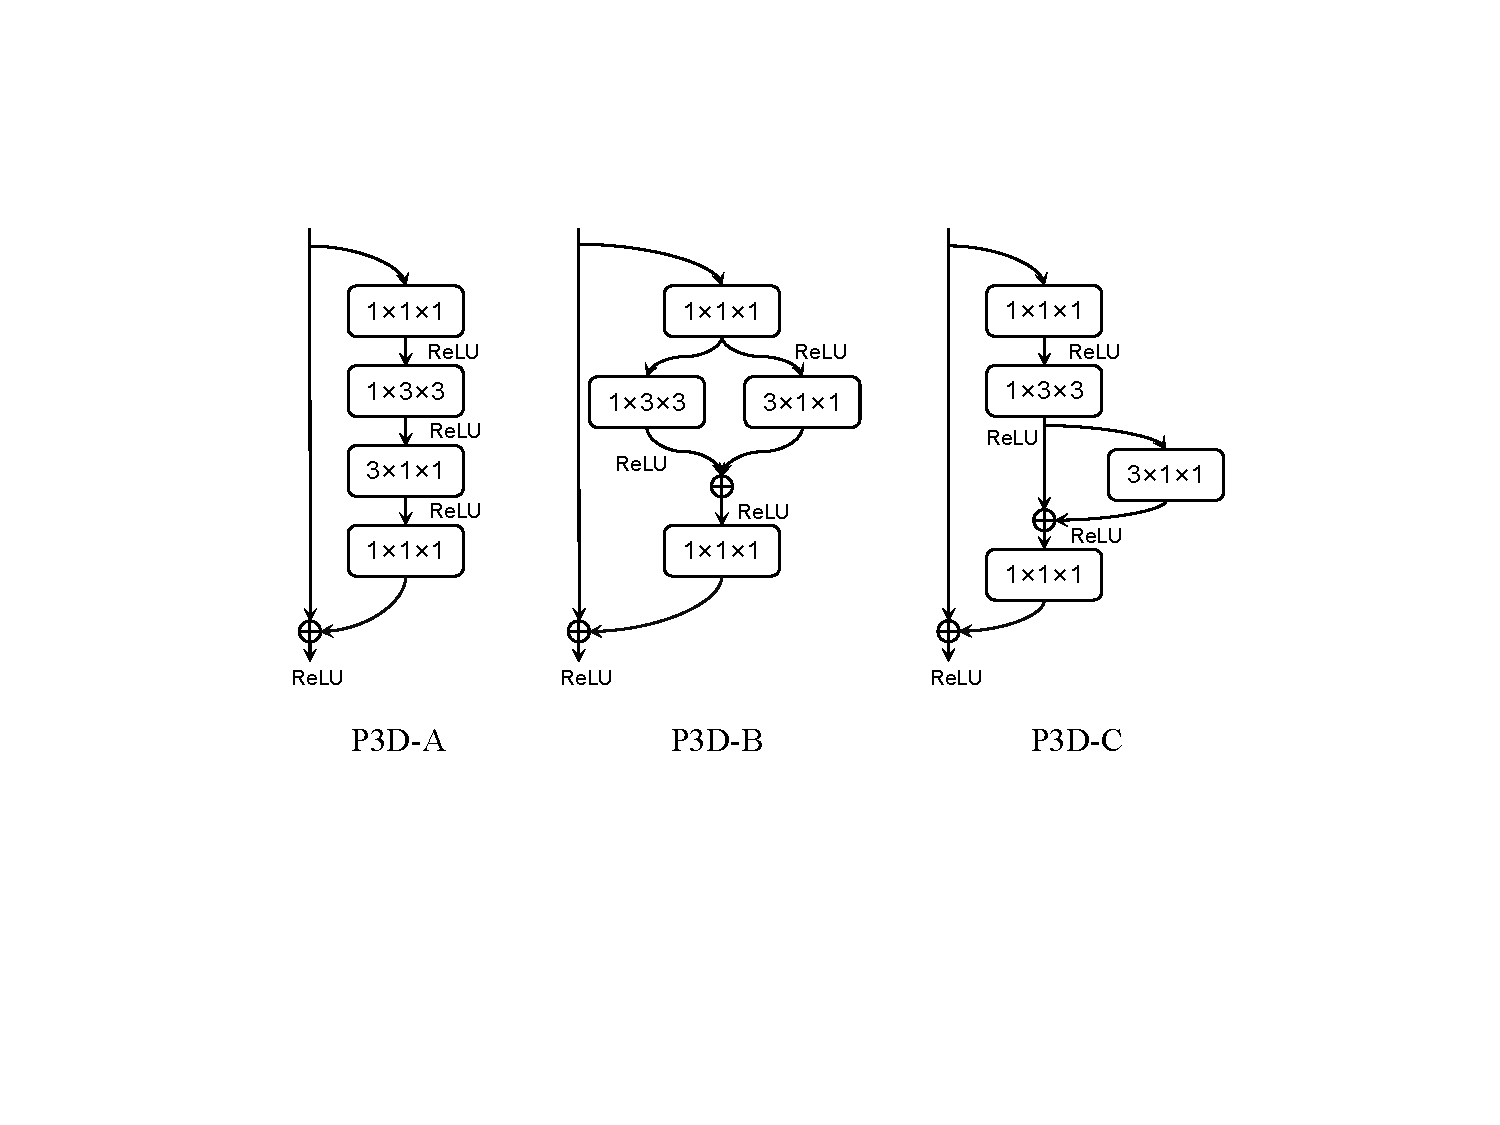
\includegraphics[width=0.75\textwidth]{P3D0}
\caption{伪3D残差网络三种设计模型}
\label{fig18}
\end{figure}

\subsection{1}

% 包含ucasthesis文档类的定义文件和配置文件,通过对它们的修改可以实现特定的模版设定。若需更新模板,一般只需用新的样式文件替换旧的即可。
%
% \begin{enumerate}
%     \item ucasthesis.cls:文档类定义文件,论文的最核心的格式即通过它来定义的。
%     \item ucasthesis.cfg:文档类配置文件,设定如目录显示为“目~录”而非“目录”。
%     \item artratex.sty: 常用宏包及文档设定,如参考文献样式、文献引用样式、页眉页脚设定等。这些功能具有开关选项,常只需在Thesis.tex中的如下命令中进行启用即可,一般无需修改artratex.sty本身。
%
%         \path{\usepackage[options]{artratex}}
%     \item artracom.sty:自定义命令以及添加宏包的推荐放置位置。
% \end{enumerate}

\subsection{2}

% 文件夹内为论文的所有实体内容,正常情况下,这也是\textbf{使用ucasthesis撰写学文论文时,主要关注和修改的一个位置,注:所有文件都必须采用UTF-8编码,否则编译后将出现乱码文本},详细分类介绍如下:
%
% \begin{itemize}
%     \item Frontpage.tex:为论文中英文封面及中英文摘要。\textbf{论文封面会根据英文学位名称如Bachelor,Master,或是Doctor自动切换为相应的格式}。
%     \item Mainmatter.tex:索引需要出现的Chapter。开始写论文时,可以只索引当前章节,以快速编译查看,当论文完成后,再对所有章节进行索引即可。
%     \item Chap{\_}xxx.tex:为论文主体的各个章节,可根据需要添加和撰写。
%     \item Appendix.tex:为附录内容
%     \item Backmatter.tex:为发表文章信息和致谢部分等。
% \end{itemize}

\subsection{3}

% 用于放置论文中所需要的图类文件,支持格式有:.jpg, .png, .pdf。其中,\verb|ucas_logo.pdf|为国科大校徽。不建议为各章节图片建子目录,即使图片众多,若命名规则合理,图片查询亦是十分方便。

\section{实验设置及分析}

\subsection{1}

% \begin{enumerate}
%     \item ref.bib:参考文献信息库。
%     \item gbt7714-xxx.bst:符合国标的文献样式定义文件。由 \href{https://github.com/zepinglee/gbt7714-bibtex-style}{zepinglee}  开发,并满足最新国标要求。与文献样式有关的问题,请查阅开发者所提供的文档,并建议适当追踪其更新。
% \end{enumerate}
\subsection{2}

\subsection{3}

\section{总结}
